\documentclass[UTF8, 12pt, oneside]{ctexart}

\usepackage[font=small, labelsep=space, labelformat=default]{caption}   % 控制浮动体标题的格式
\usepackage[left=3.0cm, right=2cm, top=2.5cm, bottom=2.5cm]{geometry}   % 页边距
\usepackage{booktabs}                    % 排版三线表
\usepackage{multirow}                    % 支持合并多行单元格
\usepackage{enumerate}                   % item
\usepackage{amsmath, amsthm, amssymb}    % 数学公式相关
\usepackage{fouriernc}                   %fourier 风格数学字体,配合 New Century Schoolbook 正文字体
\usepackage{graphicx}                    % 插入图片相关
\usepackage{subfigure}
\usepackage{float}                       %为浮动体提供不浮动的 H 模式;提供自定义浮动体结构的功能
\usepackage{fancyhdr}

\linespread{1.5}  % 1.5倍行间距

%name选项中不要使用中文逗号
\ctexset{section={name={第,章 }, format={\bfseries\zihao{3}}, aftername={\enspace}, beforeskip={24bp}, afterskip={18bp}}}  % 一级标题样式
\ctexset{subsection={format={\raggedright\zihao{-3}},aftername={\enspace},beforeskip={12bp},afterskip={6bp}}}          % 二级标题样式
\ctexset{subsubsection={format={\raggedright\zihao{4}},aftername={\enspace},beforeskip={12bp},afterskip={6bp}}}        % 三级标题样式

\captionsetup[table]{name=表.}      % 表格样式
\captionsetup[figure]{name=图.}     % 图片样式

\title{\fontsize{36pt}{12pt}\textbf{这里是封面标题}}    % 标题: 字体36磅,行距12磅, 加粗
\author{高飞}                                          % 作者
\date{\today}                                          % 日期

%%%%%%%%%%%%%%%%%%%%%%%%%%%%%%%%%%%%%%%%%%%%%%%%%%%%%%%%%%%%%%%%%%%%%%%%%%%%%%%%%%%%%%%%%%%%%%%%%%%%%%%%%%%%
\begin{document}
\maketitle
\thispagestyle{empty}

\newpage  % 新页
\tableofcontents   % 目录页
\pagestyle{empty}

\newpage           % 新页
\pagestyle{fancy}
\setcounter{page}{1} 
\section{Hello 中国}
中国位于东亚地区。

\subsection{Hello 北京}
北京,简称“京”,古称燕京、北平,是中华人民共和国首都、省级行政区、直辖市、国家中心城市、超大城市,国务院批复确定的中国政治中心、文化中心、国际交往中心、科技创新中心。截至2018年,全市下辖16个区,总面积16410.54平方千米,2019年末,常住人口2153.6万人,城镇人口1865万人,城镇化率86.6\%,常住外来人口达794.3万人。

\subsubsection{Hello 海淀区}
海淀区,隶属于北京市,位于北京城区西部和西北部,东与西城区、朝阳区相邻,南与丰台区毗连,西与石景山区、门头沟区交界,北与昌平区接壤。面积431平方千米,边界线长约146.2千米,南北长约30千米,东西最宽处29千米,约占北京市总面积的2.6\%。区境介于北纬39°53′—40°09′,东经116°03′—116°23′之间。

\paragraph{著名大学:}
\begin{enumerate}
	\item 清华大学 \\
	      学校前身清华学堂始建于1911年,校名“清华”源于校址“清华园”地名,是清政府设立的留美预备学校,其建校的资金源于1908年美国退还的部分庚子赔款。
	\item 北京大学 \\
	      北京大学创立于1898年维新变法之际,初名京师大学堂,是中国近现代第一所国立综合性大学,创办之初也是国家最高教育行政机关。
	\item 北京航空航天大学 \\
	      北京航空航天大学创建于1952年,时名北京航空学院,由当时的清华大学、北洋大学、厦门大学、四川大学等八所院校的航空系合并组建,1988年4月改名为北京航空航天大学。
\end{enumerate}

\paragraph{著名景点}:
\begin{itemize}
	\item 颐和园
	\item 圆明园
	\item 玉渊潭
\end{itemize}

\subsubsection{Hello 朝阳区}
\begin{description}
	\item[特点一] 中心城区中面积最大的
	\item[特点二] 重要的外事活动区
\end{description}

朝阳区,隶属于北京市。位于北京市的东部,西与东城区、丰台区、海淀区相毗邻,北连昌平区、顺义区,东与通州区接壤,南与大兴区相邻,幅员面积470.8平方千米,平均海拔34米,是北京市中心城区中面积最大的一个区。

\begin{table}[htbp]                % 排版优先顺序:h-当前位置,t-页面顶部,b-页面底部,p-跨页面
	\centering                         % 表格居中
	\caption{主要数据}\label{maindata}
	\begin{tabular}{l c c c c c}       % l-左对齐,c-居中,r-右对齐
		\toprule[1.5pt]                      % 表格顶部横线(1.5pt宽)
		\multirow{2}{*}{\textbf{Strain}} & \multicolumn{5}{c}{\textbf{Growth Media}}                                 \\
		\cmidrule(l){2-6}
		                                 & 1                                         & 2     & 3     & 4     & 5     \\ % Column names row
		\midrule % In-table horizontal line
		GDS1002                          & 0.9                                       & 0.821 & 0.356 & 0.682 & 0.801 \\ % Content row 1
		NWN652                           & 0.981                                     & 0.891 & 0.527 & 0.574 & 0.984 \\ % Content row 2
		PPD234                           & 0.915                                     & 0.936 & 0.491 & 0.276 & 0.965 \\ % Content row 3
		JSB126                           & 0.828                                     & 0.827 & 0.528 & 0.518 & 0.926 \\ % Content row 4
		JSB724                           & 0.916                                     & 0.933 & 0.482 & 0.644 & 0.937 \\ % Content row 5
		\midrule % In-table horizontal line
		\midrule % In-table horizontal line
		Average Rate                     & 0.920                                     & 0.882 & 0.477 & 0.539 & 0.923 \\ % Summary/total row
		\bottomrule[1.5pt]               % 表格底部横线(2pt宽)
	\end{tabular}

\end{table}

\subsection{图片}
狼伴归途,最精彩的就是宏大的史前场景再现,让人看了非常的享受,被其所征服。故事的情节还是比较的简单,年轻的孩子在失去父母呵护之后,通过自己的和狼的努力,经历千辛万苦最后回到了父母的怀抱。狼和孩子一起,最终平安到家,并为部落带来了狼这种动物,我想之后就是被驯化成狗。
\begin{figure}[ht]
	\centering
	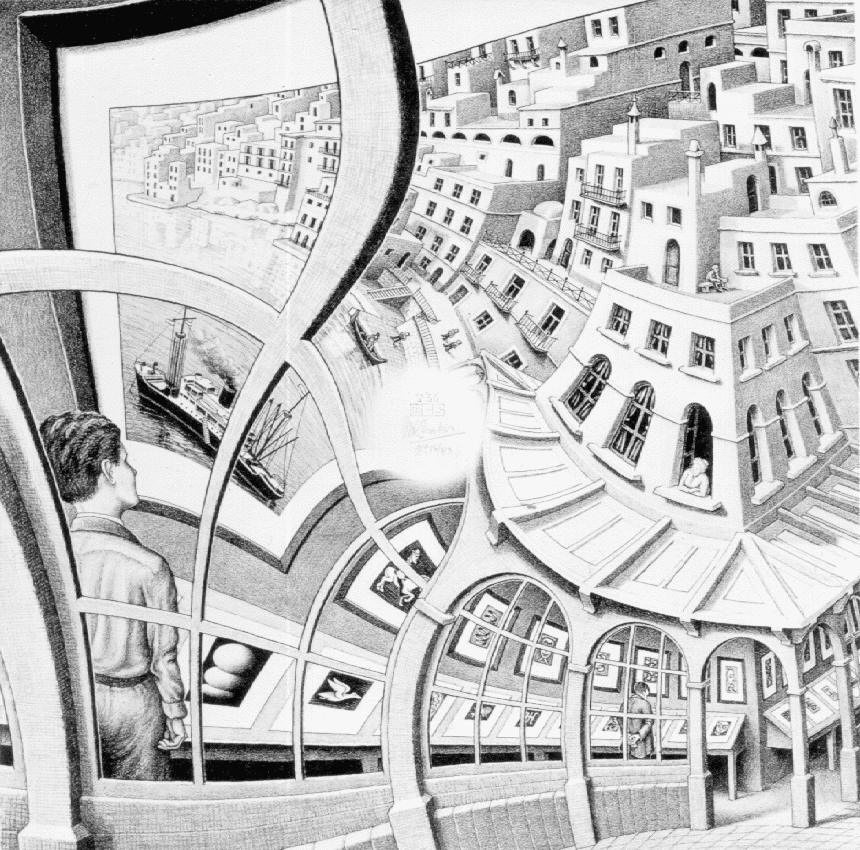
\includegraphics[width=0.75\textwidth]{Figures/GalleriaStampe}   % 0.75倍显示图片大小
	\caption{GalleriaStampe}\label{woGalleriaStampelf}
\end{figure}

\begin{figure}[ht]
	\centering
	\subfigure{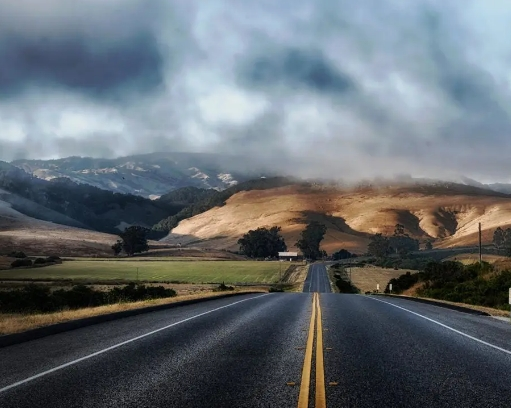
\includegraphics[width=6.0cm,height=6.0cm]{Figures/road}}
	\subfigure{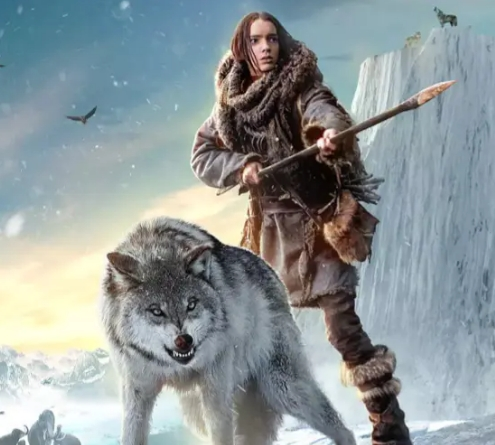
\includegraphics[width=6.0cm,height=6.0cm]{Figures/wolf}}  \\
	\vspace{-0.3cm}
	\subfigure{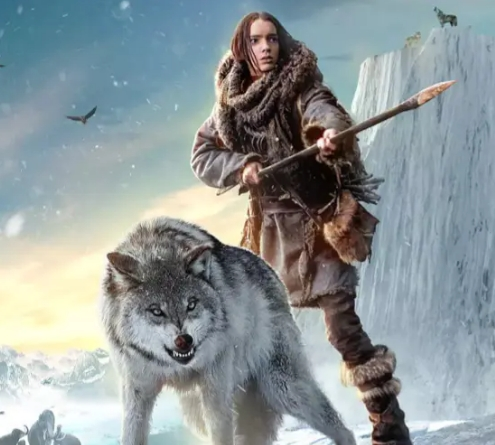
\includegraphics[width=6.0cm,height=6.0cm]{Figures/wolf}}
	\subfigure{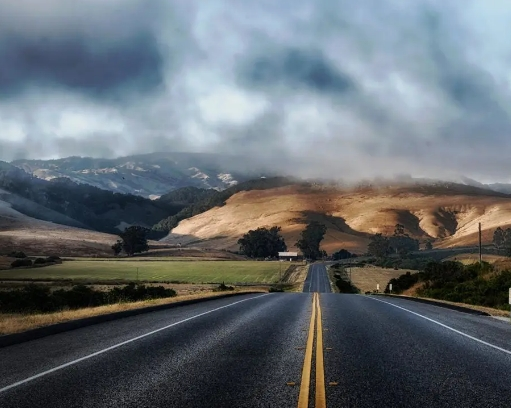
\includegraphics[width=6.0cm,height=6.0cm]{Figures/road}}
	\caption{狼伴归途场景}\label{wolf2}
\end{figure}

\end{document}